\documentclass[conf]{new-aiaa}
%\documentclass[journal]{new-aiaa} for journal papers

\usepackage[utf8]{inputenc}
\usepackage{graphicx}
\usepackage{amsmath}
\usepackage[version=4]{mhchem}
\usepackage{siunitx}
\usepackage{longtable,tabularx}
\usepackage{float}
\usepackage{subfig}

\setlength\LTleft{0pt} 

\title{Designing an Arduino-based Rocket Flight Computer for Embedded Systems Education\ }

\author{Joseph T. Telaak}
\affil{University of South Carolina, Columbia, SC, 29201, US}

\author{Dr. Wout De Backer}
\affil{Associate Professor, Ronald E. McNAIR Center for Aerospace Innovation and Research, University of South Carolina, Columbia, SC, 29201, US}

\begin{document}

\maketitle

\begin{abstract}
As amateur model rockets get more advanced, flight computers are included. They offer many benefits and enable users to include more advanced features like data logging, location tracking, thrust vector control (TVC), delayed ignition charge activation, and active component actuation. Of-the-shelf flight computers can be quite expensive, but may offer few customization options. This may lead to budget challenges for amateur rocketry projects. Working directly with complex hardware and low-level software can be intimidating for most, so development boards have been created to make amateur projects more accessible. Therefore, there is a desire to develop a low-cost flight computer suitable for all budgets, which is where microcontroller platforms like Arduino excel. The Arduino platform has many community resources and easy-to-use software, like the Arduino IDE. An inexpensive, full-featured, and modifiable Arduino-based rocket flight computer was designed based on the Arduino Mega microcontroller. This computer is compatible with the Arduino IDE as well as the standard Arduino Hardware Abstraction Layer (HAL). Common sensors like an accelerometer, barometer, and altimeter can provide the user with many different options for flight data logging and active control. On-board memory was also included to store flight data. In addition, the computer can drive high-power components like servos and ignition charges. To make software development more accessible for beginners, a comprehensive software package simplifies access to many of the sensors, communication, and external components, and a simple programming interface can be used to extract the data. Examples of certain control algorithms, like TVC, were developed to demonstrate their capabilities to users. 
\end{abstract}

\section{Introduction}
\lettrine{W}hen designing an amateur rocket, a flight computer is necessary to collect sensor data and operate active components of the rocket. As an example, if you want to actively deploy a parachute at a certain altitude, you need to be able to read the pressure data to determine altitude, process that data to check for the correct activation altitude, and then activate the charge. There are many commercial options available for users to choose from, but these options can be very expensive. These computers also offer limited options for both the hardware and software customization. Some of these computers can cost over \$300 (See Table \ref{tab:computers} for a comparison). These prices are outside of some budgets, so many users attempt to develop their own flight computers instead. Designing your own flight computer offers many opportunities to educate users in circuit design, EDA software, embedded systems programming, and algorithmic design. Getting started in the process of building your own computer can be intimidating, there are many factors to consider and many possibilities for errors that could damage components or leave you with a non-working project. This leaves an opening for a flight computer that is designed to have similar features as commercial flight computers while being open-source, extensible, and user-friendly. The design files will also be available if a user wants to build it themselves. The following sections describe the rationale behind the design choices, the implementation of the components, the software drivers, compares this computer to existing commercial computers.

During the design phase of the project, multiple existing flight computers were used as a reference to select the most desirable features. Computers like the BPS.space Signal\cite{bpssignal} and the TeleMetrum\cite{telemetrumapogee} are examples of common computers with multiple useful features beyond the basic parachute deployment\cite{easyminiapogee} (See Table \ref{tab:computers} for a comparison). Components like an IMU, barometer, and GPS were used in this computer as they have useful applications in amateur rocketry like recovery, data collection, location tracking, thrust vector control (TVC), and motor characterization. These sensors are also often found on commercial computers. After going through the process of selecting a specific sensor model, the MPU-6050\cite{mpu6050} was chosen as the IMU, the MPL3115\cite{mpl3115} as the barometer, and the L76-M33 as the GPS\cite{l76m33}. See Section \ref{sec:design} for the component selection and Section \ref{sec:commercial} for the component comparison criteria. Besides the sensors, the computer also includes the ability to control 3 servos for TVC and 6 igniter channels for state separation and recovery. The whole system was designed around a popular microcontroller platform, and after reviewing multiple options, the Arduino was chosen. Specifically the Arduino MEGA and its ATmega2560 microcontroller\cite{megadescription} were used. See Table \ref{tab:arduino} and Section \ref{subsec:dev} for a comparison on different microcontrollers. Everything is included on a custom circuit board designed to have a similar footprint to the Arduino MEGA. This computer also supports the standard Arduino Integrated Development Environment (IDE) and comes with an extension of the Arduino Hardware Abstraction Layer (HAL) to offer support for the specific components included in the system.

\section{Design Criteria}
\label{sec:design}

 When creating the flight computer, there are several factors that influence the overall design. This computer is intended to be used as an extensible educational project, so it is important to choose components with an existing user base. These components are usually found on breakout boards that can be easily purchased online and are often used in other projects. With many user examples, there are often reference schematics we can use to design the overall computer's schematic. This also simplifies the software design process as there are likely libraries to reference. SparkFun and Adafruit are manufacturers that produce breakout boards for sensors and other components\cite{mpu6050sparkfun, bmp280adafruit}. Since users will often use these in future projects, this allows users to familiarize themselves with these components and then apply them to other projects in the future. 

\subsection{Processor and Development Board}
\label{subsec:dev}

The first part of designing the flight computer is deciding which microcontroller ecosystem to base the computer on. Two popular microcontroller platforms are the STM32 and the Arduino. While the STM32's 32-bit architecture, higher performance, and advanced IO is attractive\cite{whystm}, it may be over complicated for beginners and has a development environment that is more suited for experienced engineers. Its STM32CubeIDE offers many advanced features like code generation and peripheral configuration\cite{stmcube}. Arduino's IDE is significantly more user friendly as it uses standard peripheral configurations and handles much of the configuration itself using its HAL and purpose-built language\cite{arduinoide,arduinolang}. With thousands of amateur projects based around the Arduino, it is the optimal choice for an educational project\cite{whyarduino}.

Arduino.cc offers several options for development boards, all of which are open source. Three of their most popular boards include the Micro\cite{microdescription}, UNO\cite{unodescription}, and the MEGA\cite{megadescription}. The boards are largely similar, but most of their differences come in their available IO and form factor. Comparing the 3 options (See Table \ref{tab:arduino}), the MEGA appears to be the best-suited for the computer. It has the most SRAM and IO out of the 3 options. With this computer utilizing multiple sensors, the number of IO pins and the amount of SRAM is important. 

 \begin{table}[H]
 \caption{\label{tab:arduino} Arduino Development Board Comparison}
 \centering
 \begin{tabular}{lcccccc}
 
 \hline Name\footnotemark[1] & MCU & SRAM & IO & UART & SPI & I2C\\ \hline

 Uno\cite{unodescription} & ATmega328P\cite{atmega328p} & 2Kb & 14 Digital, 6 Analog & 1 & 1 & 1\\
 Micro\cite{microdescription} & ATmega32u4\cite{atmega32u4} & 2.5Kb & 20 Digital, 12 Analog & 1 & 1 & 1\\
 Mega\cite{megadescription} & ATmega2560\cite{atmega2560} & 8Kb & 54 Digital, 16 Analog & 4 & 1 & 1\\
 
 \hline
 \end{tabular}
 \end{table}

 \footnotetext[1]{Clock speed, EEPROM, and SRAM size were not compared in this table as all 3 processors run at 16MHz, have 256Kb of flash, and 4Kb of EEEPROM\cite{microdescription, unodescription, megadescription}.}

\subsection{IMU}

In rocket flight computers, it may be necessary to include a sensor to track the acceleration and orientation of the rocket. This is a necessary function when running TVC on a rocket as the orientation feedback can be used to correctly aim the rocket. This data can provide the user with a valuable insight into how their rocket is moving while it is in flight. The accelerometer can be used for motor characterization and can tell the user the maximum force the rocket is experiencing. Gyroscopes are used for tracking the orientation of a device and its angular velocity. These sensors are commonly used in rocket flight computers to track the orientation of the rocket in flight. Usually, accelerometers, gyroscopes, and magnetometers are included on a single chip called an IMU. Magnetometers can be used to find the orientation of the rocket relative to Earth's atmosphere. 

In this computer, the MPU-6050 IMU was chosen for its average accuracy\cite{mpu6050} and its availability as a common SparkFun breakout board\cite{mpu6050sparkfun}. 

 \begin{table}[H]
 \caption{\label{tab:imus} Comparison of Common IMUs}
 \centering
 \begin{tabular}{lcccccc}
 
 \hline Name & Manufacturer & Breakout & Accuracy & Degrees of Freedom\footnotemark[1] \\ \hline

 MPU-6050\cite{mpu6050} & InvenSense & Sparkfun\cite{mpu6050sparkfun} & ±16g, ±2000deg/sec, ±1\%drift & 6\\
 MPU-9250 & InvenSense & Sparkfun\cite{mpu9250sparkfun} & ±16g, ±2000deg/sec, ±1\%drift & 9\\
 ADXL375\cite{adxl375} & Analog Devices & Analog Devices\cite{adxl375adevices} & ±200g & 3\\
 BMX160 & Bosch & dfrobot\cite{bmx160dfrobot} & ±16g, ±2000deg/sec, ±1\%drift & 9\\
 
 \hline
 \end{tabular}
 \end{table}

 \footnotetext[1]{6 degrees of freedom corresponds to a 3 axis gyroscope and a 3 axis accelerometer. 3 degrees of freedom refers to an accelerometer only in this chart. 9 degrees of freedom has the same as 6 degrees of freedom but also includes a digital compass/magnetometer.}

\subsection{Barometer}

In a flight computer, barometers are used to track the atmospheric pressure which can be used to determine altitude. Pressure is inversely proportional to altitude referenced to sea level. So as the rocket reaches a higher altitude, the pressure decreases. A lookup table can be used to estimate altitude above or below sea level at a given pressure. Users can use this data to track the max altitude the rocket reaches in flight. Common computers also use this to determine when to deploy the recovery parachute. In this computer, activation altitude and charge ignition can be customized.

In this computer, the MPL3115 was chosen specifically for its included altimeter module\cite{mpl3115}. It is also available as a breakout board\cite{mpl3115adafruit}. This allows it to calculate the altitude without external processing or calibration.

 \begin{table}[H]
 \caption{\label{tab:barometers} Comparison of Common Barometers}
 \centering
 \begin{tabular}{lcccccc}
 
 \hline Name & Manufacturer & Breakout & Accuracy (P) & Accuracy (m) & Features\\ \hline

 MS5607\cite{ms5607} & TE Connectivity & Parallax\cite{ms5607parallax} & 1 & 0.2 & Altimeter\\
 MPL3115\cite{mpl3115} & NXP & Adafruit\cite{mpl3115adafruit} & 1.5 & 0.3 & Altimeter and temperature\\
 BMP280\cite{bmp280} &  Bosch & Adafruit\cite{bmp280adafruit} & 1 & 1 & N/A \\
 
 \hline
 \end{tabular}
 \end{table}

\subsection{GPS}

GPS devices are uncommon in most entry level computers and usually unnecessary unless the rocket is expected to land at a large distance away from the launch point. GPS can be used to track the rocket's location on Earth using satellites. This is useful if the user wants to find the landing location or how far the rocket travelled over the ground. In this computer, the GPS is only enabled once the rocket is no longer in motion. GPS devices are usually limited in their maximum acceleration\cite{l76} to avoid the use in missiles or weaponry.
In this computer, the L76-M33 GPS was chosen for its quick acquisition time and its ability to use multiple GPS networks simultaneously.

 \begin{table}[H]
 \caption{\label{tab:table2} Comparison of GPS}
 \centering
 \begin{tabular}{lcccccc}
 
 \hline Name & Manufacturer & Breakout & GNSS & Aquisition (s) \\ \hline

 MAX-8Q\cite{max8q} & u-blox & No & GLONASS, GPS, and QZSS & 30\\
 L76-M33\cite{l76} & Quectel & No & GPS, GLONASS, BeiDou, Galileo and QZSS & 15\\
 
 \hline
 \end{tabular}
 \end{table}

 \subsection{Storage}

 Many flight computers do not include the ability to log flight data. Logging flight data is essential if a user wants to review any sensor data after the flight is completed. This allows the user to view information like the maximum altitude the rocket has reached or its maximum acceleration. The data can also be plotted for more insight into how the rocket behaved over time. To record the data, both a flash chip and SD card are used. The flash chip records the data in real time and the SD card is used to dump all fight data after the rocket has finished flying in order to transfer data to a laptop or other computer. A standard SD card can be used in this computer. The flash used is a W25Q64 64Mb SPI flash chip\cite{w25q64}.

 \subsection{Telemetry}

 In order to provide the user with real-time data and control, it is necessary to include a form of telemetry. Common communication methods found in commercial flight computers include Bluetooth (BT), 900Mhz/LoRa, and 70cm HAM (See Table \ref{tab:computers}). 70cm HAM requires a specific license\cite{telemegaapogee, telemetrumapogee}, so it will not be considered as since this is computer is intended for beginners and amateurs. Bluetooth has a higher bandwidth but a shorter range than LoRa, but as we are not streaming large amounts of data, we will use LoRa for its range. In this system will will use the EBYTE E220\cite{e220}.

\section{Design Process}
\label{sec:designing}

To make the computer more compact and replaceable, the entire flight computer was created on a single printed circuit board in the EasyEDA EDA software. EasyEDA allows a web-based environment for users to create their own schematics and PCBs. It is also user friendly and allows for collaboration so users can recreate the computer if they wish\cite{easyeda}. In this design, many of the schematics for the existing breakout boards of these components were used as reference when designing the computer. The Arduino MEGA reference schematic was also used to duplicate all of the same pin assignments from the original board and insure that the ATmega2560 functions the same as if it were in the MEGA board. This way, the software that is written for this computer will also work if a regular Arduino MEGA is connected to breakout boards. 

\subsection{Microcontroller}

Since this computer is essentially an Arduino reference board with peripherals that are built directly on to the board, we will use the same ATmega2560 microcontroller and ATmega16U2 serial processor. We also use Arduino's recommended designs for the power supply, reset switch, clock, and USB port\cite{mega}. The ATmega operates at a 5V logic level but much of the sensors that are used operate at 3V so logic level conversion will be required (See Fig. \ref{fig:ll_schematic}).

\begin{table}[H]
 \caption{\label{tab:pinout} Digital I/O Pin Assignment for Peripherals}
 \centering
 \begin{tabular}{ccc|ccc}

 \hline Component & GPIO & Name & Component & GPIO & Name \\ \hline

 Flash SD & PB1 & SCK & GPS & PD2 & UART1 RX\\
 Flash SD & PB2 & MOSI & GPS & PD3 & UART1 RX\\
 Flash SD & PB3 & MISO & IMU + Barometer & PD0 & SCL\\
 Buzzer & PA6 & 28 & IMU + Barometer & PD1 & SDA\\
 Flash CS & PC7 & 30 & SD CS & PC6 & 31\\
 Gyro Rail & PC5 & 32 & Baro Rail & PC4 & 33\\
 Buzzer Rail & PC3 & 34 & LoRa CS & PC2 & 35\\
 Servo1 & PA0 & 22 & Servo2 & PA1 & 23\\
 Servo3 & PA2 & 24 & Servo4 & PA3 & 25\\
 Servo5 & PA4 & 26 & Servo6 & PA5 & 27\\
 
 \hline
 \end{tabular}
 \end{table}

\pagebreak
\subsection{Sensors}

For both the MPU-6050 IMU and MPL3115 Barometer, the schematics from the breakout boards were replicated in the computer\cite{mpu6050sparkfun, mpl3115adafruit}. The included regulators on the boards were not included as the logic level conversion is handled by another component. Other than the main chip, both breakout boards contain mostly decoupling capacitors and pull-up resistors for the I2C bus.

\begin{figure}[H]%
    \centering
    \subfloat[\centering IMU]{{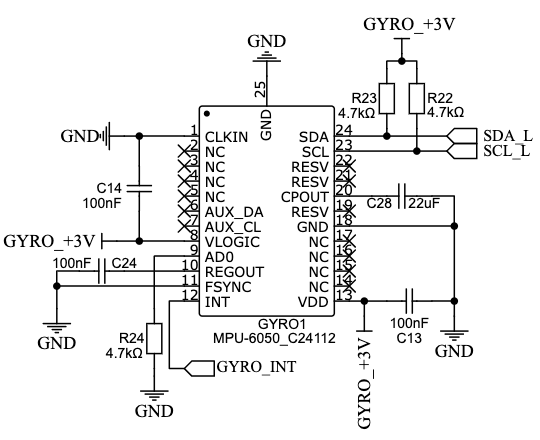
\includegraphics[scale=0.35]{imu_schematic.png} }}%
    \qquad
    \subfloat[\centering Barometer]{{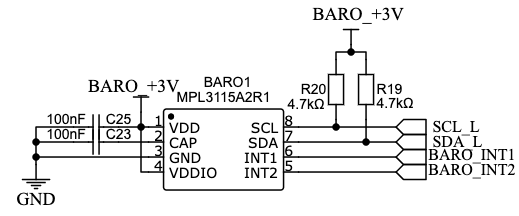
\includegraphics[scale=0.35]{baro_schematic.png} }}%
    \caption{IMU and Barometer Schematics}%
    \label{fig:imuandbaro}%
\end{figure}%

The L76 GPS does not have a breakout board but is instead a SoC that contains all the necessary components to perform its functions\cite{l76}. It only requires decoupling capacitors and a connection to reset, which in this case is pulled high. An LED is also attached for the PPS indicator.

\begin{figure}[H]
    \centering
    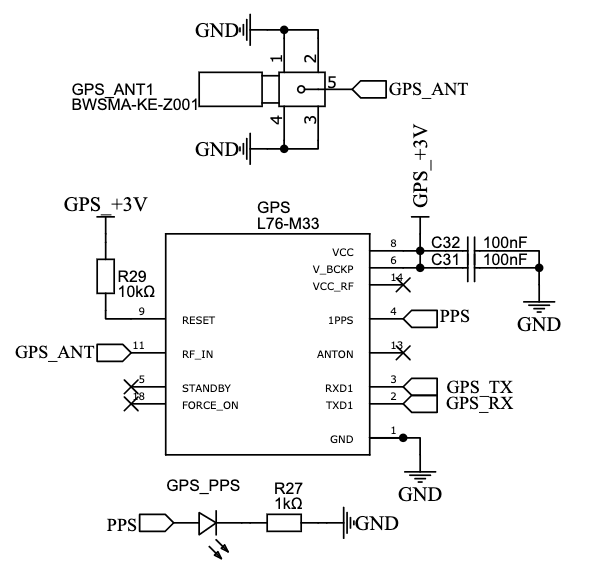
\includegraphics[scale=0.35]{gps_schematic.png}
    \caption{GPS Schematic}
    \label{fig:gps_schematic}
\end{figure}

\pagebreak
\subsection{Servos and Igniters}

To control charges or igniters, it is not necessary for a dedicated IC. Actuation of these can usually be achieved by a simple arrangement of components to control the high current flow (See Fig. \ref{fig:pyro_schematic}). In this case, we are using a MOSFET to act as a switch to connect the charge to ground. The MOSFET does require a resistor in series with its gate to drop the voltage. It also requires a pull-down resistor to ground as MOSFETs have a small capacitance between its drain and gate, and this needs to be dissipated\cite{ao3400}.

\begin{figure}[H]
    \centering
    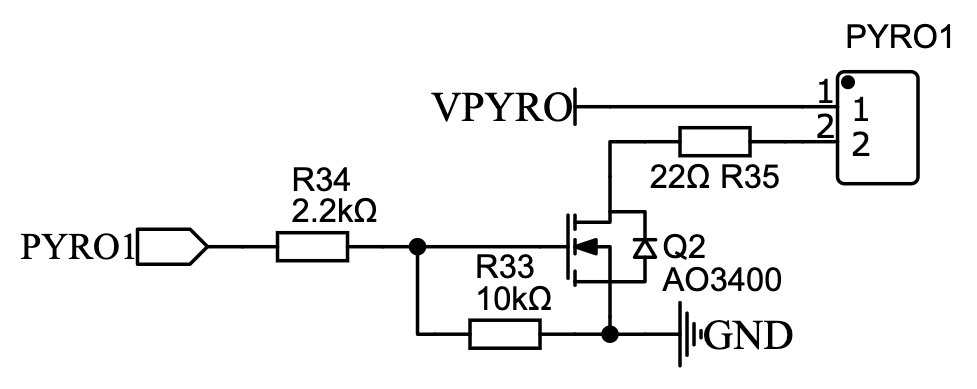
\includegraphics[scale=0.25]{pyro_schematic.png}
    \caption{Charge Actuator Schematic}
    \label{fig:pyro_schematic}
\end{figure}

\subsection{Load Switches}

Since this computer has a number of external sensors and peripherals, depending on the application and user requirements, some may not be used. For example, the GPS is only used to track the location of the rocket once it has landed. It is not necessary for the GPS to operate in flight due to government limitations\cite{l76}, so it is powered off in flight. Each sensor IC is connected to an individual load switch responsible for disconnecting the IC's power. By default, the sensors are disconnected from power unless the user initializes them. This saves power and reduces the chance for errors and unexpected behavior to occur.

\begin{figure}[H]
    \centering
    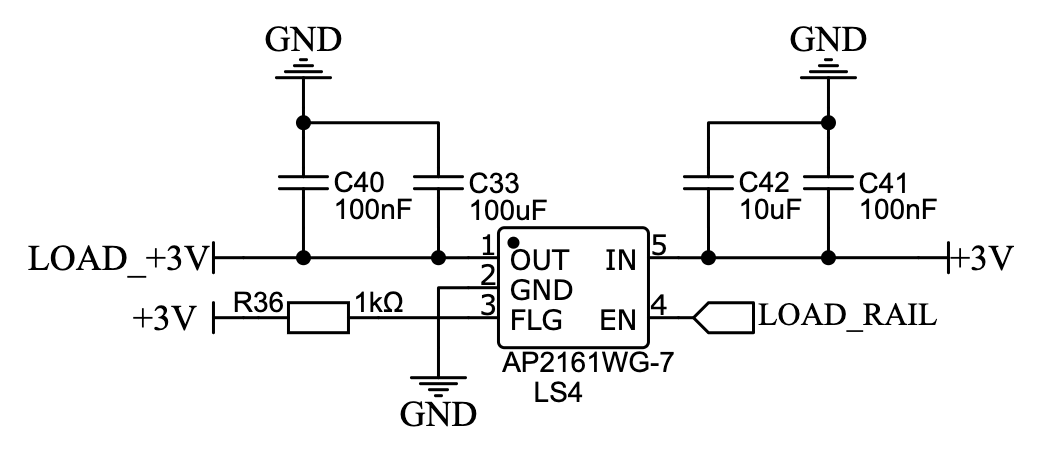
\includegraphics[scale=0.25]{loadsw_schematic.png}
    \caption{Load Switch Schematic}
    \label{fig:loadsw_schematic}
\end{figure}

\pagebreak
\subsection{Logic Level Conversion}

To avoid damaging the components, the 5V logic level from the ATmega2560\cite{atmega2560} needs to be converted to the 3V that the sensors use. Some of these devices are tolerant of 5V or 3V, but to be within the recommended range, the levels are going to be shifted to 3V in this computer. This is done with a TXS0108 chip\cite{txs0108}. Decoupling capacitors are placed on both the 3V and 5V rails. The output enable is pulled high through a jumper and pulled low when the jumper is disconnected.

\begin{figure}[H]
    \centering
    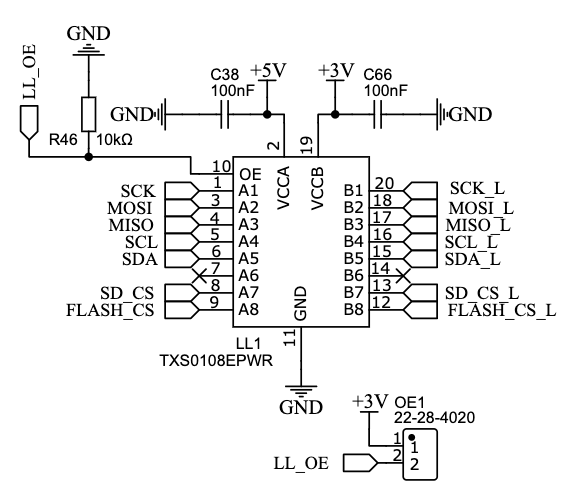
\includegraphics[scale=0.35]{ll_schematic.png}
    \caption{Logic Level Converter Schematic}
    \label{fig:ll_schematic}
\end{figure}

\subsection{Storage and Telemetry}

Many SD cards use SPI to communicate by default, so nothing needs to be added other than the card holder. The SPI flash chip only requires the SPI connection, decoupling capacitors, and the hold and write-protect signals\cite{w25q64}. The E220 Lora module also uses the same SPI communication as the flash chip\cite{e220}.

\begin{figure}[H]
    \centering
    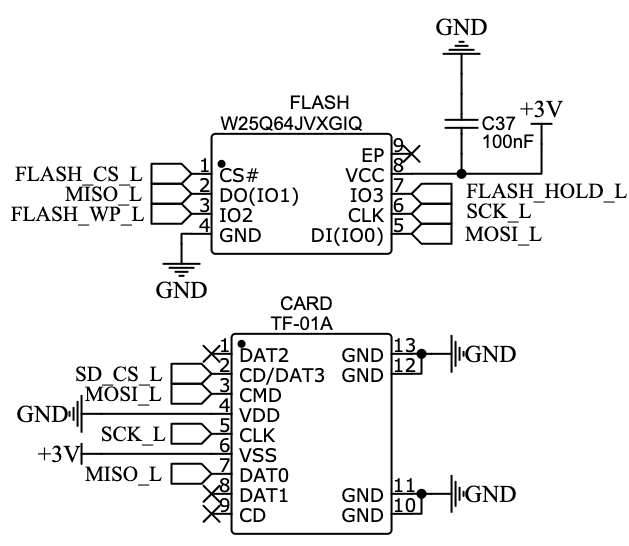
\includegraphics[scale=0.35]{storage_schematic.png}
    \caption{Storage Schematic}
    \label{fig:storage_schematic}
\end{figure}

\subsection{Safety}

To reduce the chances for accidents to occur, there are two switch terminals included on the board. One terminal is for the main power switch that disconnects power to the entire computer. The other terminal is for arming the ignition charges. This helps prevent unintended ignition do to software or hardware errors.

\section{Software}

In order to read the sensor data and perform functions, it is necessary for the flight computer to include a software package. Since this computer is designed to use standard Arduino code, we can reuse much of the Arduino HAL. The Arduino Hardware Abstraction Layer (HAL) is used as an interface between the user and the code necessary to operate the microcontroller and to interact with the hardware registers for IO control. We can build off this Arduino HAL and create our own system. Instead of including the "Arduino.h" header file when writing code, we can include our custom header file. In our HAL, we have access to the standard functions and a wrapper around the libraries for the sensors. As an example, we will have dedicated functions to pull data from each sensor without having to understand which IO port and protocol that is required for that device. The libraries and protocol information to enable communication with each component are included in their datasheets. These protocols are then implemented in the new HAL. Initialization is handled just like the original Arduino HAL. Components can be selectively enabled and disabled by controlling their power rails.

\section{Comparison to Commercial Computers}
\label{sec:commercial}

Using EasyEDA's bill-of-materials (BOM) tool, then total cost for this computer comes out to around \$75\footnotemark[1]. This is priced significantly lower than the basic flight computers that are compared in Fig. \ref{tab:computers} and costs 600\% less than a higher-end computer.

 \begin{table}[H]
 \caption{\label{tab:computers} Hardware Comparison}
 \centering
 \begin{tabular}{lcccccc}
 
 \hline Name & Price (est) & MCU & Charges & Sensors & Telemetry & Other\\ \hline
 
 Signal\cite{bpssignal} & \$349 & ATSAMD21 & 3 & IMU, Barometer & BT\footnotemark[2] & TVC \\
 AVA\cite{ava} & N/A\footnotemark[3] & 3 Independent & 6 & IMU, GPS, Barometer & BT + LoRa & TVC \\
 EasyMini\cite{easymini} & \$102\cite{easyminiapogee} & LPC11U14 & 2 & Barometer & N/A & Buzzer \\
 EasyMega\cite{easymega} & \$358\cite{easymegaapogee} & STM32L151 & 4 & IMU, Barometer & N/A & Buzzer \\
 TeleMetrum\cite{telemetrum} & \$382\cite{telemetrumapogee} & STM32L151 & 2 & IMU, GPS, Barometer & 70cm ham & Buzzer \\
 TeleMega\cite{telemega} & \$508\cite{telemegaapogee} & STM32L151 & 4 & IMU, GPS, Barometer & 70cm ham & TVC, Buzzer \\
 This computer & \$75\footnotemark[1] & ATmega2560 & 4 & IMU, GPS, Barometer & LoRa & TVC, Buzzer \\
 
 \hline
 \end{tabular}
 \end{table}

 When looking at the above chart, it can be seen that this computer is comparable to the BPS.space Signal and TeleMega, but at a significantly reduced price. The BPS.space Signal offers TVC and has some software customization but has a more complicated software package. This computer is priced in the same range as a simple computer that only offers a barometer for recovery charge deployment.

\footnotetext[1]{The price varies depending on component prices and minimum order quantity. This price was calculated using the individual unit price instead.}
\footnotetext[2]{Bluetooth is shortened to "BT"}
\footnotetext[3]{This flight computer is not in production}

\section{Conclusion}

In this paper, we went through the process of selecting components for creating a flight computer that is user-friendly and based on the Arduino platform. We were able to design a device that had more features that expensive computers while staying in the price range of budget computers with minimal features. With this computer, there are many possibilities that can be explored in the future. With the basic hardware capabilities, many software features can be added to enable more complex control over a rocket. 

\pagebreak
\bibliography{sample}

\end{document}
